\documentclass{article}
\usepackage{amsmath}
\usepackage{tikz}
\title{Challenges in target archery Question 5 Attachment}
\author{Donald Leung}
\date{\today}
\begin{document}

\maketitle

\section{Modern Arrows}

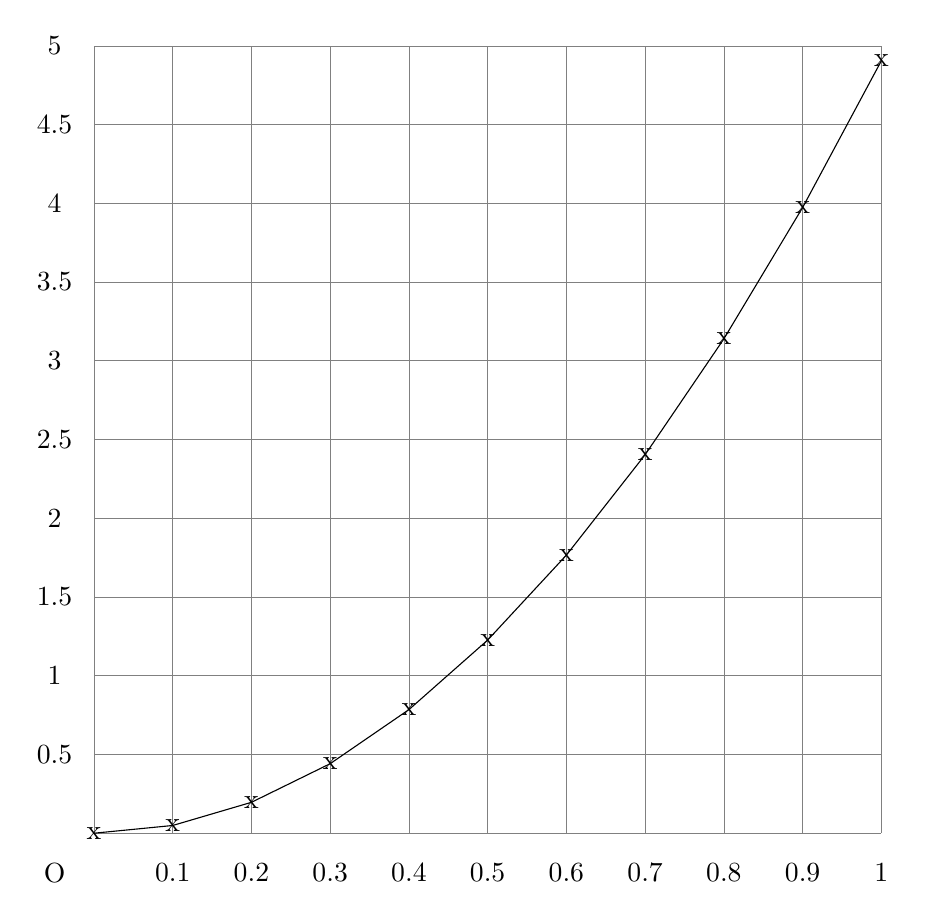
\begin{tikzpicture}
% Grid
\draw[help lines] (0,0) grid (10,10);
% Origin
\node (O) at (-0.5,-0.5) {O};
% Horizontal Axes (Time in seconds)
\node (xa1) at (1,-0.5) {0.1};
\node (xb1) at (2,-0.5) {0.2};
\node (xc1) at (3,-0.5) {0.3};
\node (xd1) at (4,-0.5) {0.4};
\node (xe1) at (5,-0.5) {0.5};
\node (xf1) at (6,-0.5) {0.6};
\node (xg1) at (7,-0.5) {0.7};
\node (xh1) at (8,-0.5) {0.8};
\node (xi1) at (9,-0.5) {0.9};
\node (xj1) at (10,-0.5) {1};
% Vertical Axes (Vertical Displacement in metres)
\node (ya1) at (-0.5,1) {0.5};
\node (yb1) at (-0.5,2) {1};
\node (yc1) at (-0.5,3) {1.5};
\node (yd1) at (-0.5,4) {2};
\node (ye1) at (-0.5,5) {2.5};
\node (yf1) at (-0.5,6) {3};
\node (yg1) at (-0.5,7) {3.5};
\node (yh1) at (-0.5,8) {4};
\node (yi1) at (-0.5,9) {4.5};
\node (yj1) at (-0.5,10) {5};
% Points on the graph
\node (gd10) at (0,0) {x};
\node (gd11) at (1,0.0981) {x};
\node (gd12) at (2,0.3924) {x};
\node (gd13) at (3,0.8829) {x};
\node (gd14) at (4,1.5696) {x};
\node (gd15) at (5,2.4525) {x};
\node (gd16) at (6,3.5316) {x};
\node (gd17) at (7,4.8069) {x};
\node (gd18) at (8,6.2784) {x};
\node (gd19) at (9,7.9461) {x};
\node (gd110) at (10,9.81) {x};
% Connecting the Dots (not allowed in Physics but nevermind :p)
\draw (0,0) -- (1,0.0981);
\draw (1,0.0981) -- (2,0.3924);
\draw (2,0.3924) -- (3,0.8829);
\draw (3,0.8829) -- (4,1.5696);
\draw (4,1.5696) -- (5,2.4525);
\draw (5,2.4525) -- (6,3.5316);
\draw (6,3.5316) -- (7,4.8069);
\draw (7,4.8069) -- (8,6.2784);
\draw (8,6.2784) -- (9,7.9461);
\draw (9,7.9461) -- (10,9.81);
\end{tikzpicture}

The graph above shows the vertical displacement changing with time for a range of $60$ metres for an arrow at speed $60 ms^{-1}$ (modern arrows) that is shot \emph{horizontally}.  The downwards direction is considered positive displacement in this case.  The vertical axis is vertical displacement in meters while the horizontal axis is time in seconds.

\emph{Note: I used ``connect the dots'' approach in this software to draw the curve of best fit only because I don't really know how to draw a quadratic in this software.}

\section{Arrows from 5 Decades Ago}

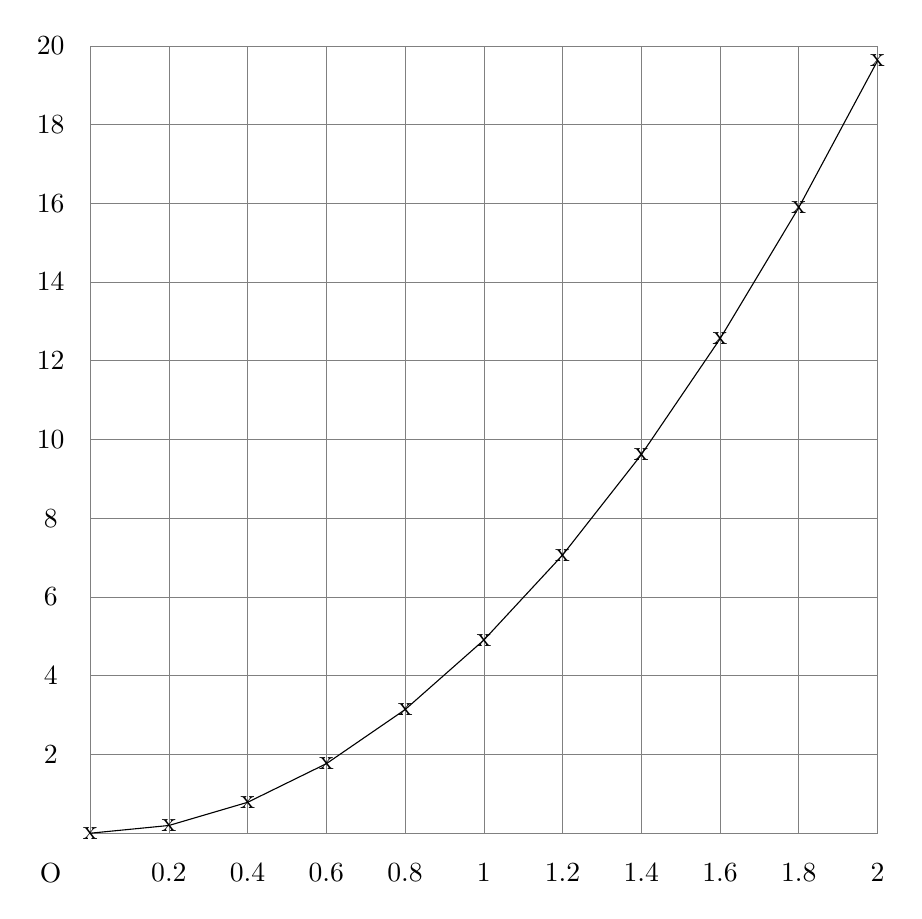
\begin{tikzpicture}
% Grid
\draw[help lines] (0,0) grid (10,10);
% Origin
\node (O) at (-0.5,-0.5) {O};
% Horizontal Axes (Time in seconds)
\node (xa1) at (1,-0.5) {0.2};
\node (xb1) at (2,-0.5) {0.4};
\node (xc1) at (3,-0.5) {0.6};
\node (xd1) at (4,-0.5) {0.8};
\node (xe1) at (5,-0.5) {1};
\node (xf1) at (6,-0.5) {1.2};
\node (xg1) at (7,-0.5) {1.4};
\node (xh1) at (8,-0.5) {1.6};
\node (xi1) at (9,-0.5) {1.8};
\node (xj1) at (10,-0.5) {2};
% Vertical Axes (Vertical Displacement in metres)
\node (ya1) at (-0.5,1) {2};
\node (yb1) at (-0.5,2) {4};
\node (yc1) at (-0.5,3) {6};
\node (yd1) at (-0.5,4) {8};
\node (ye1) at (-0.5,5) {10};
\node (yf1) at (-0.5,6) {12};
\node (yg1) at (-0.5,7) {14};
\node (yh1) at (-0.5,8) {16};
\node (yi1) at (-0.5,9) {18};
\node (yj1) at (-0.5,10) {20};
% Points on the Graph
\node (gd20) at (0,0) {x};
\node (gd21) at (1,0.0981) {x};
\node (gd22) at (2,0.3924) {x};
\node (gd23) at (3,0.8829) {x};
\node (gd24) at (4,1.5696) {x};
\node (gd25) at (5,2.4525) {x};
\node (gd26) at (6,3.5316) {x};
\node (gd27) at (7,4.8069) {x};
\node (gd28) at (8,6.2784) {x};
\node (gd29) at (9,7.9461) {x};
\node (gd210) at (10,9.81) {x};
% Connect the dots
\draw (0,0) -- (1,0.0981);
\draw (1,0.0981) -- (2,0.3924);
\draw (2,0.3924) -- (3,0.8829);
\draw (3,0.8829) -- (4,1.5696);
\draw (4,1.5696) -- (5,2.4525);
\draw (5,2.4525) -- (6,3.5316);
\draw (6,3.5316) -- (7,4.8069);
\draw (7,4.8069) -- (8,6.2784);
\draw (8,6.2784) -- (9,7.9461);
\draw (9,7.9461) -- (10,9.81);
\end{tikzpicture}

The graph above shows the vertical displacement changing with time for a range of $60$ metres for an arrow at speed $30 ms^{-1}$ (arrows from five decades ago) that is shot \emph{horizontally}.  The downwards direction is considered positive displacement in this case.  The vertical axis is vertical displacement in meters while the horizontal axis is time in seconds.

\emph{Note: I used ``connect the dots'' approach in this software to draw the curve of best fit only because I don't really know how to draw a quadratic in this software.}

\end{document}